\documentclass[12pt]{proposalnsf}
\usepackage[usenames]{color} %used for font color
\usepackage{amssymb} %maths
\usepackage{amsmath} %maths
\usepackage{graphicx}
\usepackage{hyperref}
\usepackage{epsfig}

\newcommand{\GeV}{\ensuremath{\mathrm{GeV}}}
\newcommand{\TeV}{\ensuremath{\mathrm{TeV}}}
\newcommand{\GeVc}{\ensuremath{\mathrm{GeV}}}
\newcommand{\TeVc}{\ensuremath{\mathrm{TeV}}}
\newcommand{\GeVcc}{\ensuremath{\mathrm{GeV}}}
\newcommand{\TeVcc}{\ensuremath{\mathrm{TeV}}}
\newcommand{\pt} {\ensuremath{p_\mathrm{T}}\xspace}
\newcommand{\kt}            {\ensuremath{k_\mathrm{T}}\xspace}
\newcommand{\antikt}        {anti-\kt}
\newcommand{\ttbar}        {\ensuremath{\mathrm{t}\overline{\mathrm{t}}}}
\newcommand{\bbbar}        {\ensuremath{\mathrm{b}\overline{\mathrm{b}}}}
\newcommand{\qqbar}        {\ensuremath{\mathrm{q}\overline{\mathrm{q}}}}


\DeclareFontFamily{OT1}{psyr}{}
\DeclareFontShape{OT1}{psyr}{m}{n}{<-> psyr}{}
\def\times{{\fontfamily{psyr}\selectfont\char180}}


\renewcommand{\refname}{\centerline{References cited}}


% this handles hanging indents for publications
\def\rrr#1\\{\par
\medskip\hbox{\vbox{\parindent=2em\hsize=6.12in
\hangindent=4em\hangafter=1#1}}}

\def\baselinestretch{1}



\begin{document}

\title{High Energy Physics Research at the CMS Experiment }

% >> Authors
\author{Salvatore Rappoccio, PhD.}

% >> Date
\date{\today}




\maketitle

\abstract{
The first run of the Large Hadron Collider (LHC) in Geneva,
Switzerland has
completed with resounding success after the discovery of a Higgs boson
at 125 \GeVcc. This particle is expected to break the symmetry between
the electroweak and electromagnetic scales of interactions. However,
with this new discovery, new questions immediately arise. It was
expected that in addition to the solution to electroweak symmetry
breaking, the first run of the LHC would also shed light onto the
question of why the electroweak scale is so much different from the
Planck scale (the hierarchy problem). No such information was
observed, however, and so the
continuation of the LHC program is critically important to our
understanding of nature at the smallest scales. 

This proposal focuses on finding solutions to the hierarchy problem
using novel reconstruction techniques to reconstruct
highly-boosted standard model particles such as top quarks, $W/Z$ and
Higgs bosons. The principle investigator (PI) has played a critical
role in bringing these techniques to deployment, and will continue to
do this in the future. 

To accomplish this goal, it is necessary to fully utilize, the
particle flow reconstruction algorithm at CMS. More generally,
particle flow been a
resounding success in the discovery of the Higgs boson at 125 \GeVcc, and
also in the myriad of searches in the first run of the LHC for
supersymmetric and other exotic models beyond the standard model. The
proposed research will bring the particle flow algorithm into the next
runs of the LHC, based on the extensive previous experience of the PI
that has been gained in the past.  

In addition to these tasks, the proposed research will also contribute
to commissioning and operations of the pixel detector at CMS. 

}


\section{Introduction}

Prof. Salvatore Rappoccio (tenure-track Assistant Professor) joined
the Faculty at the University at Buffalo, SUNY (UB) in 2012. The UB
group has an NSF grant (Award Number 1205960, July 15th 2012 - June
30th 2015) from Professors Kharchilava and Iashvili, however this was
renewed one year before Prof. Rappoccio joined the Faculty and does
not provide support for him or his group. 



Prof. Rappoccio's group consists
of Dr. James Dolen (postdoctoral fellow), Mr. Joshua Kaisen and Ms. Maral Alyari
(graduate students), Mr. Brendan Smith and Mr. Jonathan Goodrum (undergraduate
students, the latter supported under the ``Collegiate Science and
Technology Program'' (CSTEP)
at UB, which provides research funding for minority and
disadvantaged undergraduate students). Work has already started
on the proposed research using short-term startup funds. 
These startup funds will run out by 30-June-2014. If no funding is
found, the support for Dr. Dolen, Mr. Kaisen, and Ms. Alyari will run
out, and they will not be able to continue their studies. 

The larger UB group consists of Profs. Kharchilava and Iashvili, two
postdoctoral fellows, Dr. Ashish Kumar and Dr. Supriya Jain, and three
Ph.D. students, Mr. Joseph Zennamo, Mr. Andrew Godshalk, and Mr. Jimin
George. Prof. Rappoccio's group has already commenced collaboration
with the teams of Kharchilava and Iashvili, specifically in the pixel
detector commissioning. 



With the discovery of a 
standard model (SM)-like Higgs boson at
125~\GeVcc\ during the 7 and 8 \TeV\ runs of the LHC 
(``Run 1'')~\cite{higgs_atlas,higgs_cms}, 
the focus of collider physics now turns to understanding the nature of
the observed mechanism for electroweak symmetry breaking.
The SM is an effective theory, and quadratically-divergent
quantum-loop corrections to the Higgs
mass would require an enormous degree of fine tuning, if the Higgs
mass is to remain finite up to the Planck scale. This is commonly
referred to as the hierarchy problem, which can be resolved by
introducing contributions beyond the standard model (BSM). 
These BSM models must survive a myriad of precision tests of the SM
(such as the recent observation of $B_s\rightarrow
\mu^+\mu^-$~\cite{bsmumu_cms,bsmumu_lhcb}), and extensive direct
searches. 

Various mechanisms beyond the standard model
have been proposed to resolve the hierarchy problem.
Since the most divergent 
quantum correction to the Higgs mass
involves top quarks, it is natural to suppose
that these BSM mechanisms preferentially involve interactions with the
top quark to cancel this divergence.
Two major classes of models which solve the hierarchy problem
discussed above are supersymmetry
(SUSY)~\cite{Gunion:1987qv,Feng:1999mn,Kitano:2006gv,Barbieri:2009ev,Horton:2009ed}
and extra dimensions (ED)~\cite{ed,rs1,rs2,rs_gluon_1}. SUSY involves
a ``supersymmetry'' of nature, where all known particles have a
``superpartner'' of opposite spin (bosons have a fermionic partner,
and vice versa). The production of SUSY particles at the LHC typically
involves cascade decays resulting in top quarks and other light
supersymmetric and nonsupersymmetric particles. ED postulates extra
spatial dimensions, in which gravity propagates differently than the
other forces, resulting in an apparent discrepancy in our local 3+1 dimensional
manifold (or ``brane''). ED models typically involve
Kaluza-Klein (KK) excitations of known particles, and KK gluons in
particular typically decay into $\ttbar$ pairs. 
One common feature of both of these models is the presence of top
quarks in the final state which are often highly Lorentz boosted. 



In recent years, new jet-clustering techniques have been developed to handle
highly-boosted SM particles including top
quarks~\cite{Seymour:1993mx,boostedhiggs,catop_theory,catop_cms,jetpruning1,jetpruning2,nsub,heptoptagger,trimming}.
Summaries of these techniques are in Refs.~\cite{boost2010,boost2011}.
These
large jets are referred to as 
``boosted jets'' (or ``boosted tops'' in the case of top quarks), and
they are
different from jets that originate from quantum chromodynamic (QCD)
processes in that they exhibit different internal structure
(``substructure''), and have an intrinsic jet mass. 
These algorithms
analyze the substructure and mass
of the boosted jet to break it up into smaller ``subjets'' which can be
analyzed at angular scales smaller than 0.7, thereby allowing analysis
of highly-boosted states. Figure~\ref{boostedtop_eventdisplay}
shows an event display of such a highly-boosted top quark at CMS. 
The blue rectangles represent the
energy measured in the hadronic calorimeter, the green
rectangles represent the energy measured in the electromagnetic
calorimeter, and the three groups of colored lines (purple, red,
and orange) represent three different subjets as measured in
the tracker. Using traditional reconstruction techniques, this object
would be reconstructed as a single four-vector, whereas the newer
techniques involving jet substructure are able to discern the three
separate subjets. 


\begin{figure}[h!]
    \centering
    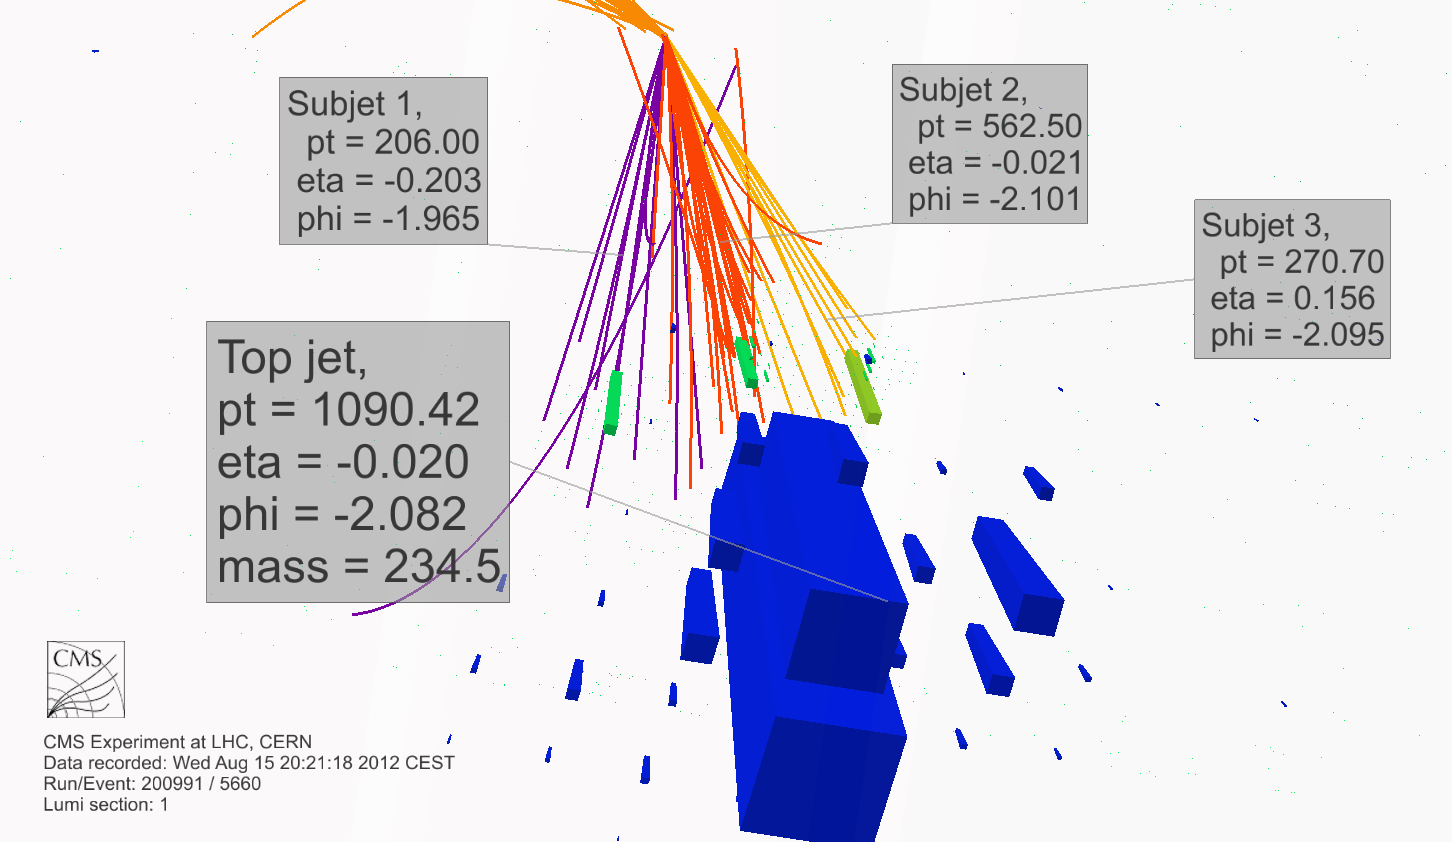
\includegraphics[width=100mm]{topjet_rechits_white}
    \caption{\label{boostedtop_eventdisplay} Event display of a
      highly-boosted top jet. The blue rectangles represent the
      energy measured in the hadronic calorimeter, the green
      rectangles represent the energy measured in the electromagnetic
      calorimeter, and the three groups of colored lines (purple, red,
      and orange) represent three different ``subjets'' as measured in
      the tracker.}
\end{figure}



\begin{figure}[h!]
    \centering
    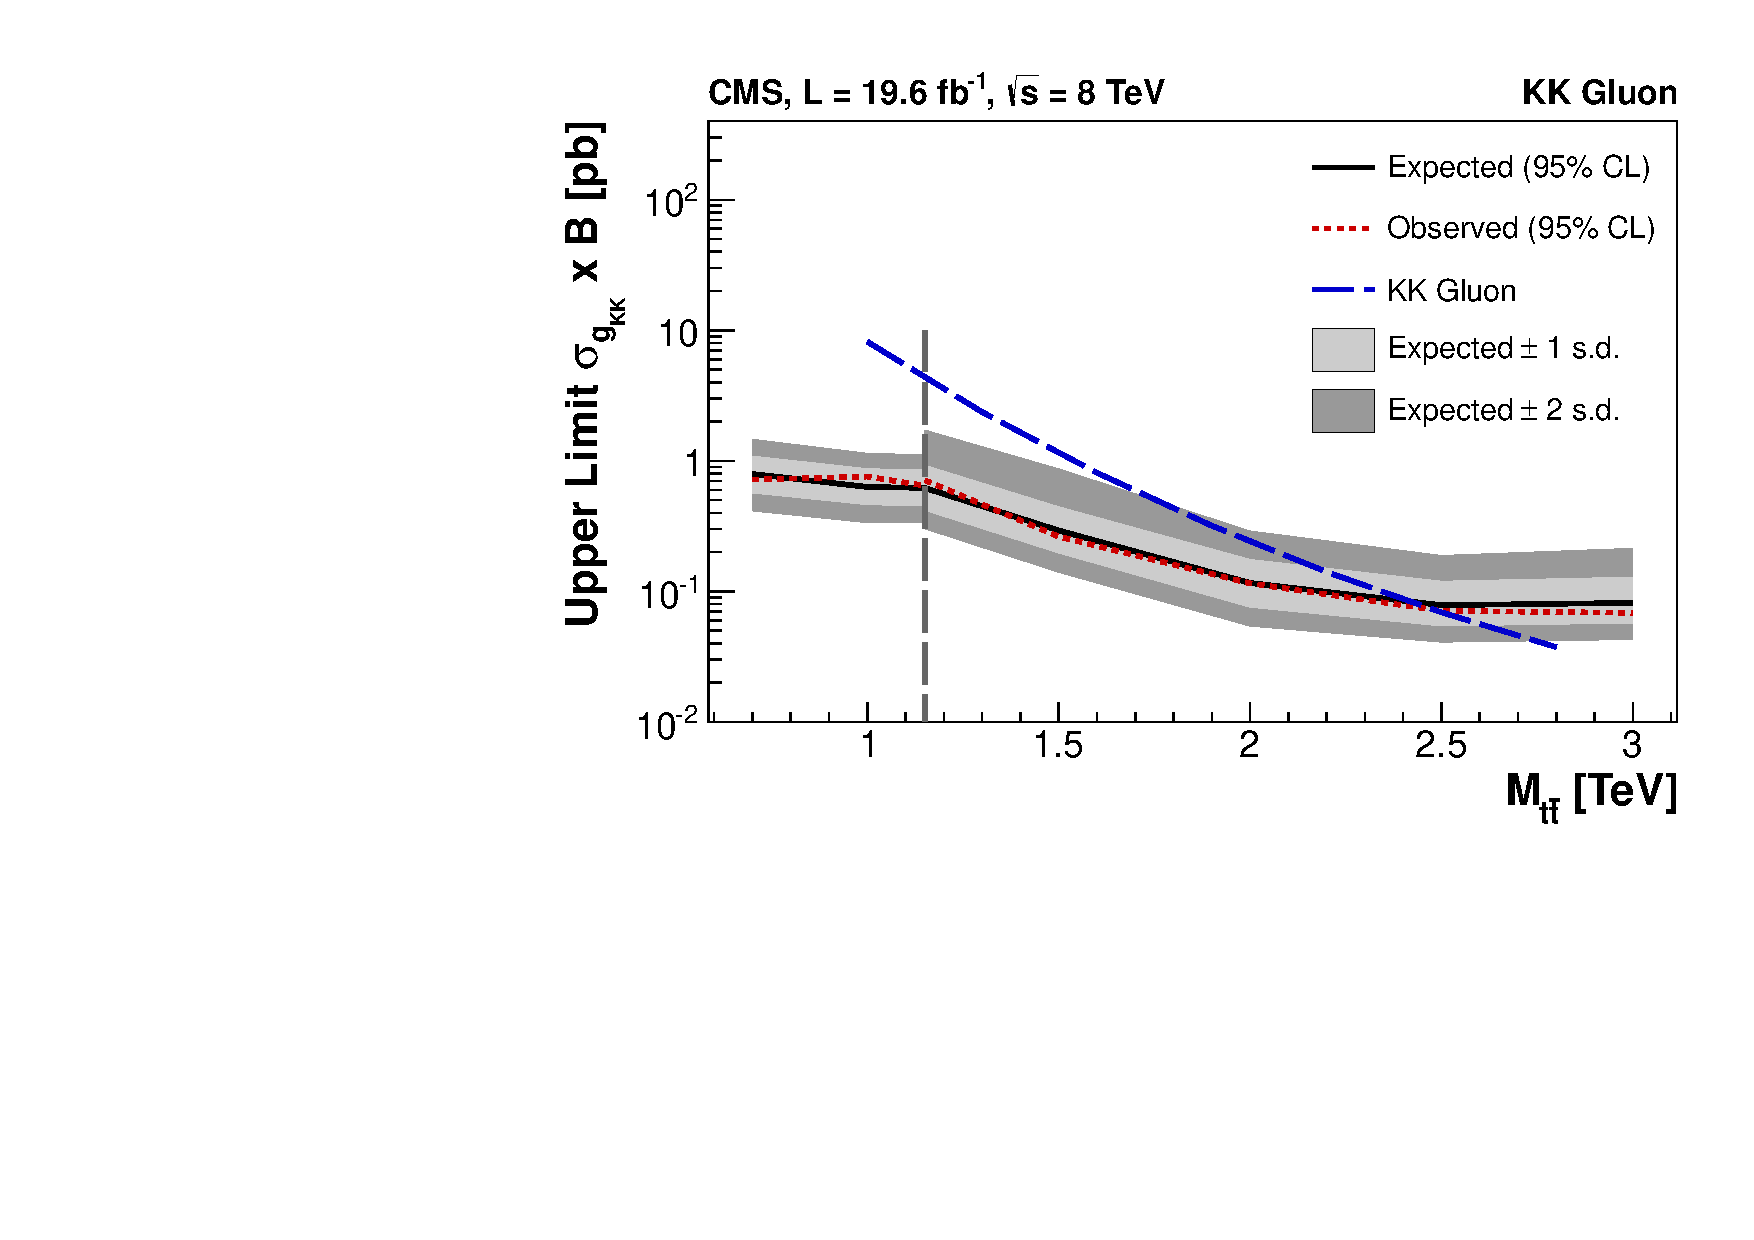
\includegraphics[width=100mm]{limits-kk_combined}
    \caption{\label{fig:limits-kk_combined}Limits on the mass of
      possible Kaluza-Klein excitations of the gluon in decays to
      $\ttbar$ pairs from a combination of results in
      Refs.~\cite{B2G-12-005,B2G-12-006}. }
\end{figure}


In both of the BSM solutions to the hierarchy problem outlined above
(SUSY and ED), the majority of the
lower masses for the new particles have been excluded. The top squark
mass is currently
constrained to be above $\sim$ 650 \GeVcc\ if the mass of the
neutralino is zero~\cite{SUS-13-011}, and the mass of
KK gluons is currently constrained to be
above $\sim$ 2.5 \TeVcc\ (Fig.~\ref{fig:limits-kk_combined}).
The Lorentz boosts of top quarks in the final state of these two cases
will be around $\gamma=4$ for the first case, and around $\gamma=7$ in
the second, which means the masses of the unexcluded particles will be
in the ``boosted regime'' in the upcoming 13 or 14 \TeV\ run of the
LHC (``Run 2'') and beyond (``Run 3''). Without using these
boosted-top strategies, the
sensitivity of searches for particles predicted by these BSM models is
reduced by a factor of ten or more, even at energies accessible during
Run 1 of the LHC. For instance, for a KK gluon with a mass of 2
\TeVcc, the sensitivity of boosted-top techniques is a factor of 10
better than the sensitivity without using these techniques. This
improvement grows even larger with the mass of the KK gluon. 


\subsection{Boosted Jet Algorithms}

The performance of the boosted-jet algorithms at CMS will be heavily
affected by increasing pileup in Run 2 and beyond. For instance,
Fig.~\ref{jetmass_toptags_trimming} is a figure made by Dr. Dolen in
the context of the ``SnowMass on the Mississippi'' Community Summer
Study~\cite{snowmass}, and shows the jet
mass of a boosted top-quark jet in three separate cases during Run 3: 
without pileup (solid histogram), with 140 pileup
interactions (open green histogram), and with 140 pileup
interactions after applying an advanced boosted jet ``grooming''
technique (the ``jet trimming'' technique~\cite{trimming}, in the open
magenta
histogram). The naive implementation of the
``Run 1''-style
algorithm to a higher pileup regime fails miserably. The major
innovation of combining strengths from different techniques, however,
can rescue the performance quite handily, and restores the jet mass
almost back to the case where there was no pileup at all. 

This is one example of a problem that was already identified and fixed
by using innovative techniques to resolve the existing problems. There
are several other major limitations that are also under investigation
which will also require a heavy amount of development to solve for Run
2 and beyond. For example, boosted-jet techniques start to break down
at very high energies because the SM particles are sufficiently
boosted that their decay products fall into one single calorimeter
cell. This could be mitigated, for instance, with a more finely-tuned
PF algorithm as described in the next section. Only through a robust
and comprehensive development and deployment strategy will these
challenges be met. 

The work outlined in this proposal includes the development of new
techniques in order to fully realize the
capability of the CMS detector in discovering new physics with boosted
jets in an environment that is increasingly difficult to analyze. The
success of this approach
will require major innovations and cutting-edge tools, as
well as a broad view of the field at large. The
previous experience of Prof. Rappoccio (cited below) has provided the expertise
needed to solve these extensive problems, and can ensure that timely
and deployable strategies can be developed prior to the startup of Run
2 of the LHC. 

\begin{figure}[h!]
    \centering
    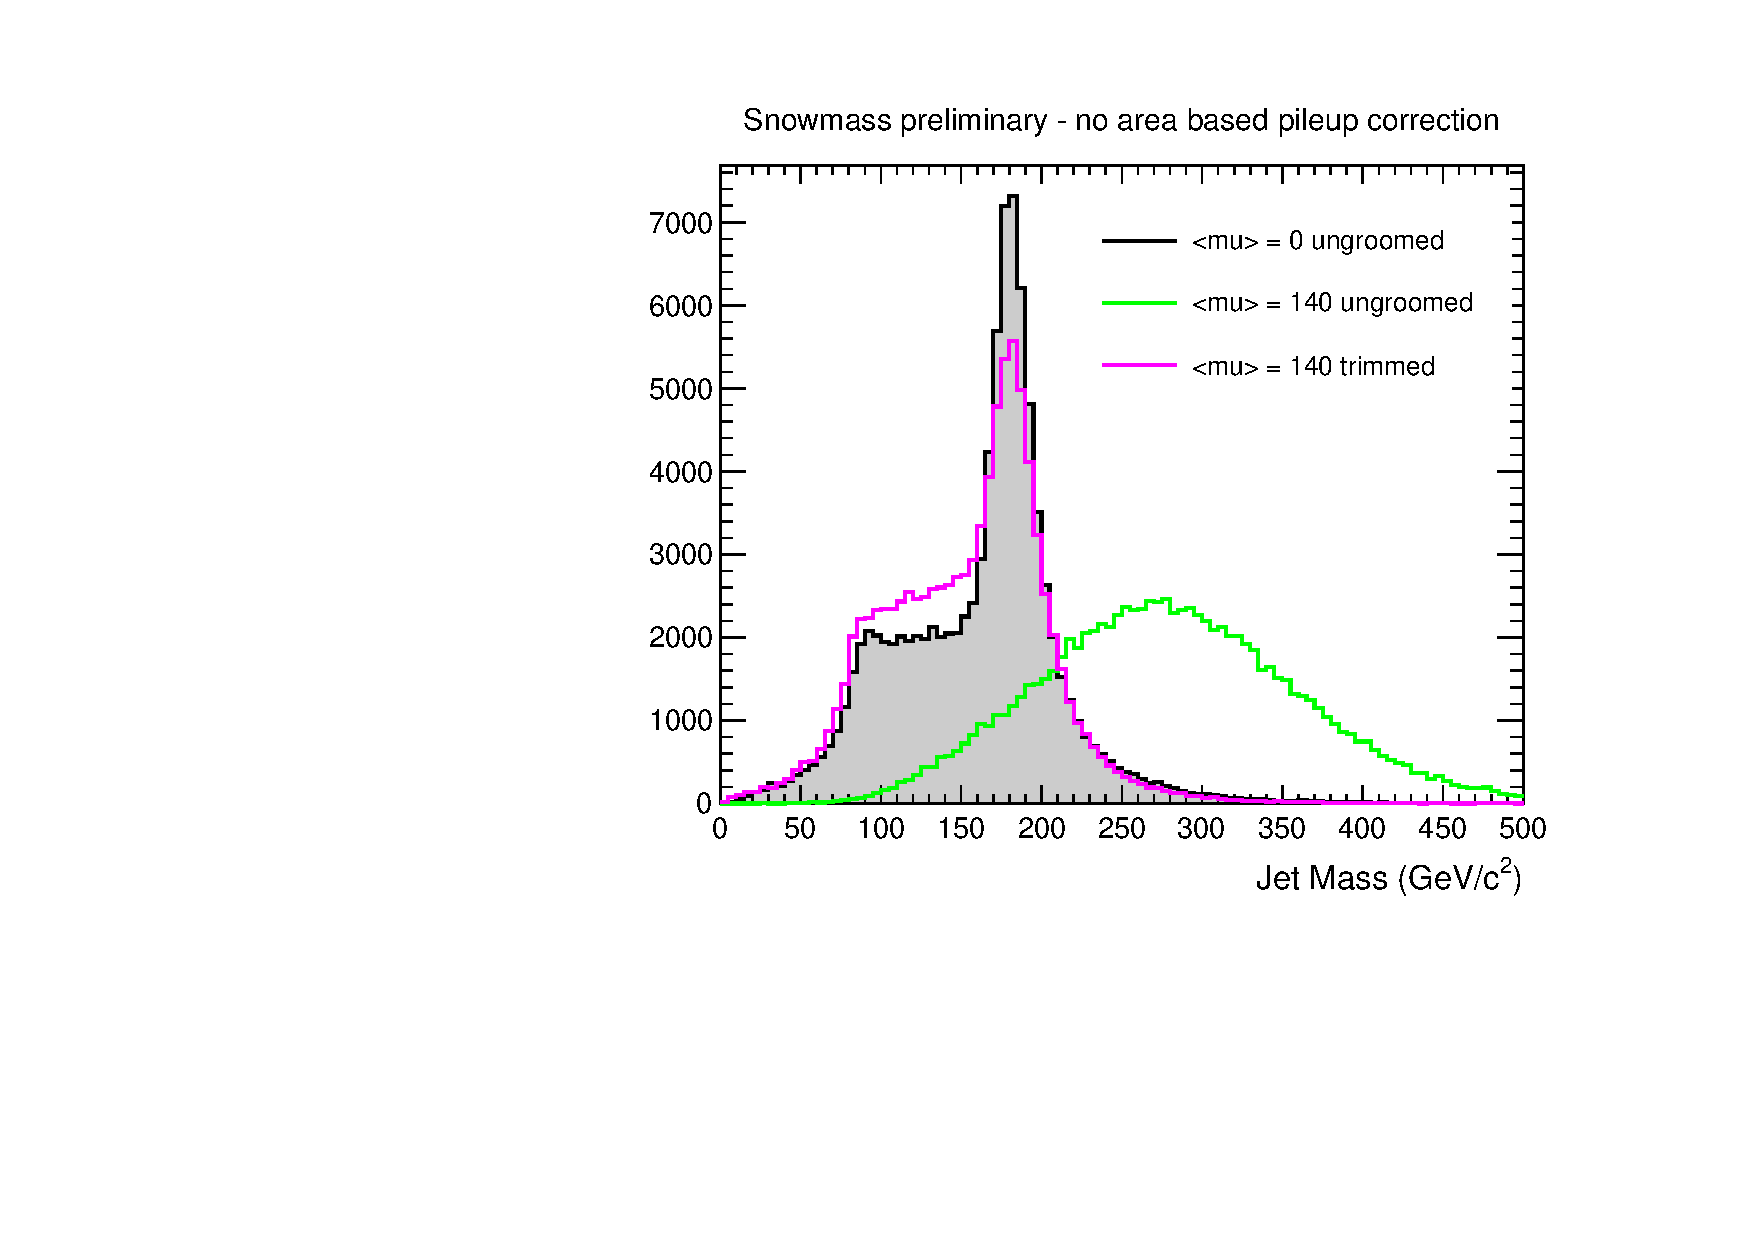
\includegraphics[width=100mm]{jetmass_toptags_trimming}
    \caption{\label{jetmass_toptags_trimming} Jet mass for boosted
      top-quark jets produced at $\sqrt{s} = 8$ \TeV. Three cases are
      shown : without pileup (solid histogram), with 140 pileup
      interactions (open green histogram), and with 140 pileup
      interactions after applying the jet trimming technique (open
      magenta histogram).}
\end{figure}


\subsection{BSM Searches with Boosted Jets}
\label{sec:bsm}

\subsection{SM Measurements with Boosted Jets}
\label{sec:topxs}


\subsection{Particle Flow}
\label{sec:pf}

The success of the general physics program at CMS during
the first run of the LHC, and in particular for the jet substructure
techniques outlined above, was heavily contingent on the
PF algorithm~\cite{particleflow}. 
When using the PF algorithm, performance of the top-tagging
algorithms at CMS was increased by 20\% compared to using calorimetric
information only, driven by the superior energy
and angular resolution of the algorithm. In addition, the PF algorithm
is capable of removing
over 60\% of pileup directly, by removing charged hadrons that are
associated to pileup vertices. This already reduces the scale of the
problem of pileup considerably, and the substructure algorithms at CMS
are heavily reliant on this technique. 

The PF algorithm, however, is heavily tuned (by construction) on the
Run 1 detector. A considerable amount of work must be done to migrate
the PF algorithm to the new detector conditions, as well as to adapt
to the enormous increase in pileup.
In the coming ``Phase 1'' and ``Phase 2''
tracker and HCAL upgrades at CMS~\cite{Dominguez:1481838,Mans:1481837}
the detector will be improved in a number of ways, including the
addition of a fourth silicon pixel layer to improve pileup
rejection, and
updates to the HCAL electronics to allow for readout of the
longitudinal segmentation of hadronic showers. These upgrades will
necessitate a second tuning of the PF
algorithm, with new opportunities and challenges directly
ahead. Mr. Kaisen and Prof. Rappoccio are already working with the
``global event description'' (GED), tracking and HCAL groups at CMS to
update the PF algorithm to take advantage of the new segmented HCAL
readout, as well as the new pixel-detector configurations. 

The success of the CMS boosted-object program is heavily
contingent on the success of the PF algorithm. Without the superior
energy and angular resolution of subjets and the pileup
reduction capabilities of the PF algorithm, the substructure
techniques we have developed will be significantly degraded.

However, with the newer detector comes new possibilities. It may be
possible to mitigate the efficiency loss of jet substructure
algorithms at very high energies (when $\gamma$ is so large that all of
the products decay in a single calorimeter cell) using the upgraded
detector capabilities. For instance, combining information from the
longitudinally-segmented
readout of the HCAL with the finer angular segmentation of the ECAL
and the trackers,
it may be possible to lessen the impact of the intrinsic
HCAL granularity. 
The upgraded CMS detector needs to be fully-utilized in order to
maximize the potential for physics discoveries. Advanced development
of the PF algorithm may illuminate new advantages that were
previously impossible.

\subsection{Trigger Development and Data Quality Monitoring}

In order to analyze highly-boosted topologies in BSM searches, 
the relevant data must be collected in efficient triggers. Furthermore, the
reconstruction, calibration, and trigger efficiencies of these
algorithms must be incorporated in the overall program of 
data-quality monitoring (DQM) at CMS. At the present time, there are
very few triggers that are capable of collecting boosted-jet
events in the upcoming Run 2, and those that do exist necessitate very
high kinematic thresholds which limit their sensitivity. This needs
immediate rectification if we are to be prepared to adequately perform
these searches for new physics with boosted objects detailed in this
proposal. 

A major difficulty here is that the jets in events in
Run 2 will be highly-polluted with pileup interactions. 
In fact, using algorithms that we have previously developed in Run 1
to deal with pileup mitigation may not continue to work in Runs 2 and
3 with
such large pileup. Since there is a large stochastic fluctuation of
the pileup background (roughly 1 \GeVc\ per jet), with 140 pileup
interactions, a 400 \GeVc\ jet will be expected to be composed of
nearly 50\% pileup. 

Rigorous and
expansive application of boosted-jet, jet-substructure, pileup
removal, and other advanced techniques
will be necessary to collect the boosted-jet datasets with reasonable
efficiency without having enormously high event rates. For instance,
if one were to select events with a jet-mass requirement, without any
corrections the trigger rate would grow linearly with the number of
pileup interactions, and without any corrections the trigger would
rapidly become untenable. However, from the studies by Prof. Rappoccio in
Ref.~\cite{SMP-12-019}, it is observed that applications of grooming
techniques to the jets can eliminate the growth of the jet mass with
increasing pileup entirely. Further investigations in this avenue of
inquiry are sure to yield extremely promising results. 


Dr. Dolen and Ms. Alyari will partake in the analysis and development
of the triggering program at CMS to ensure that boosted-jet searches
will acquire the necessary data in Run 2 without having event rates
that simply scale linearly with pileup. 
Furthermore, Ms. Alyari will be participating in the DQM of generic
and boosted jets to ensure that the algorithms are being implemented
effectively and that no adverse interactions occur unexpectedly,
thereby ensuring the safety of the physics program proposed here. 



\subsection{Forward Pixel Detector Commissioning and Operations} 

Rappoccio's group, as well as the larger UB group, are very active in
the forward pixel (FPIX) detector
commissioning for the Phase-1 upgrade. The UB group is involved with
the NSF Cooperative Agreement ``U.S. CMS Phase-1 Upgrades'', Fastlane
number 7334626, to support undergraduate students working on the
CMS Phase 1 FPIX upgrade project. 
However, this Cooperative Agreement does not provide support
for the graduate students nor postdoctoral fellows already working on
the project. 

In the past year, Rappoccio's group has begun working on the FPIX
upgrade project. Dr. Dolen is permanently stationed at Fermilab to
take advantage of the Silicon Detector (SiDet) Facility, and is
already participating in the FPIX module testing. During the
summer of 2013, the UB team (led by Dr. Dolen and Dr. Kumar)
commissioned 50 High-Density Interconnect
(HDI) boards for the FPIX modules, including visual inspection, spot
checks of the connectivity of anomalies found by this visual
inspection, and also randomized spot checks of interconnections to
ensure high quality of the produced modules. For this exercise, a
probe station was revived for usage at
SiDet, and a LabView program was developed to do the testing.

In addition to the already completed activities, Rappoccio's group has
committed to other HDI burnin tests, tests of the half-disk assembly
of the FPIX detector, beam tests (the first scheduled in Fall 2013),
and overall commissioning of the FPIX detector. Longer-term activities
will include operations and support of the upgraded Phase-1 pixel
detector once it is installed at CMS. 

Without support for Dr. Dolen and Mr. Kaisen, these proposed
activities will not be possible. 


\section{Prior Work}

\subsection{CMS Activities}

Prof. Rappoccio has played a critical leading role in implementing and
understanding these jet substructure and boosted techniques at the LHC
in general, and became the foremost expert of this topic at CMS while
a postdoctoral fellow at Johns Hopkins University working under NSF
Grant 1100862 and earlier. 
His early studies (before collision data) and
implementation of the algorithms are outlined in
Ref.~\cite{catop_cms}. He has authored the first searches
for new physics with collision data to be published using boosted
top~\cite{EXO-11-006} and boosted $W/Z$~\cite{EXO-11-095} techniques
anywhere in the world, as well as the first measurement of the jet
mass at CMS~\cite{SMP-12-019}. In addition, he has contributed to
several of the now-seminal review papers about the subject, which are
used as standard references and benchmarks in the community at
large~\cite{boost2010,boost2011}. 

After these pioneering efforts successfully established the CMS
Collaboration as a world leader in the fields of jet substructure and
boosted hadronic final states, Prof. Rappoccio
was made the convener of the ``Beyond Two Generations'' Physics
Analysis Group (B2G PAG) at CMS, which focuses on these highly-boosted
final states, in particular in the top sector. 
In his tenure as convener since August 2012, CMS has deployed these
techniques in 5 analyses of the 8 \TeV\ data (in preparation for paper 
submission)~\cite{B2G-12-005,B2G-12-006,B2G-12-012,B2G-12-015,B2G-12-019}. 
Furthermore, the techniques are being adopted in four other
analyses to search for other exotic signatures (including the 8-\TeV\
continuation of Ref.~\cite{EXO-11-095} in Ref.~\cite{EXO-12-024}), as
well as two analyses to search for supersymmetry. 

%The performance we have achieved with these algorithms is nothing
%short of astonishing. First with 7 \TeV\ collision data, and now with
%8 \TeV\ collision data, the efficiency to identify fully-merged
%top-quark jets is approximately 50\% with a misidentification rate of
%approximately 5\%, and the efficiency to identify fully-merged
%$W/Z$-boson jets is approximately 70\% with a misidentification rate
%of approximately 20\%. 
The latest 8 \TeV\ limits using boosted
techniques to search for $\ttbar$ resonances are shown in
Fig.~\ref{fig:limits-kk_combined} and finally probe, for
the first time, a viable region of parameter space available for
models of ED that are not already disfavored by
precision measurements~\cite{Davoudiasl:2009cd}. 
Without the boosted-jet strategies for searches that Prof. Rappoccio has
developed, it would not have been possible to access this regime at
CMS by any other method. This highlights the absolutely critical
nature of developing these tools in searches. 



In addition to pioneering the searches for new physics using
boosted-jet techniques, Prof. Rappoccio has also been instrumental in developing,
commissioning, and maintaining the general jet reconstruction and
particle-flow algorithms at CMS. Some of the areas in which
He has played a leading role are the development of the ``charged
hadron subtraction'' algorithm at CMS, where charged PF candidates
associated with pileup vertices were removed directly from
jets, resulting in a 10-20\% improvement in the jet energy
resolution, as well as the development of the
median-$p_\mathrm{T}$-per-unit-area pileup correction for jets at CMS. He was also
instrumental in getting the ``anti-$k_\mathrm{T}$'' algorithm~\cite{ktalg} accepted
by the CMS collaboration, and redesigned the software framework to
make usage of the {\tt fastjet} package~\cite{fastjet,fastjet1} so as to have a
common algorithmic basis for jet reconstruction in ATLAS, CMS, and the
theoretical community. He also
participated in the software validation and
data-quality monitoring (DQM) of the jets at CMS before and during the
Run 1 startup commissioning at 2.36 and 7 \TeV. 

Furthermore, Prof. Rappoccio's group has participated in the larger UB
activities of FPIX commissioning and testing during the first year of
his position. Dr. Dolen and Dr. Kumar developed tests for the FPIX
modules using a probe station at Fermilab, leading a team of graduate
and undergraduate students after severe budgetary constraints at
Fermilab descoped much of the project. 


\subsection{Non-CMS Activities}
To highlight the importance of this project, the SnowMass effort
described above has made the identification of boosted jets an
extremely high priority for the future of HEP in general. Dr. Dolen
has been extensively involved in this effort, and is co-leading the
group that focuses on boosted top-quark tagging techniques. 

In addition, Prof. Rappoccio has played an integral part of the {\bf BOOST}
conference series and other conferences, such as the {\bf Boston Jet
  Substructure Workshop}. The BOOST conference is the foremost
conference on jet substructure and boosted-jet algorithms, and the
conference reports in 2010 and 2011 are used as standard references in
benchmarking these techniques~\cite{boost2010,boost2011}.


As a graduate student at Harvard University, Rappoccio also performed
major updates and modifications of the Silicon Readout Controller
(SRC) for the CDF experiment at Fermilab. These developments allowed
the readout of the silicon detector at Level 1 of the CDF triggering
system, which then could be passed to a tracking algorithm at Level
2. This made the extensive $B$-physics program at CDF possible, since
without these track triggers, the quality of results would have been
severely degraded. 


\clearpage


\clearpage
\section{Outreach and education}
\label{sec:outreach}


While it is critical to pursue a rigorous research program, a large
part of the responsibility of scientists is to educate the next
generation effectively. There is already extensive work being done to
educate high school-level students and teachers via the {\em QuarkNet}
program  at UB, however there is
very little in the way of educating the general
public. 
The plan outlined in this proposal will extend the coverage of the
outreach program at UB to engage the broader
public in discussions of major results in particle
physics, as well as to enliven particle physics for young students. 
This will be implemented based on similar events as the
``HiggsFest''~\cite{higgsfest} that Prof. Rappoccio organized at UB. 


\subsection{Higgsfest and other public events}

The ``Higgsfest'' that was organized here at UB in 2012
is highlighted in Ref.~\cite{higgsfest}. The aim of the event was to
invite the general public for ``plain English'' summaries and hands-on
demonstrations that were geared for a multitude of age and knowledge
levels. 
This was attended by over 100 people, including children,
high-school students, physics and non-physics undergraduates, and
interested members of the community. 

Some of the hands-on demonstrations included building models of
Feynman diagrams from craft material (for young children), a
fully-functional four-layer coincidental muon scintillator detector,
a cloud chamber made out of tupperware, felt, and dry ice, and the
actual Higgs events from the CMS collaboration in an interactive event
display. 
The event was covered by the ``UB Reporter'' here at
UB~\cite{higgsfest_ubreporter}. 

Two more such events are proposed, the first to coincide with the LHC
turn-on sometime in 2015, and the second to coincide with the newest
results from the LHC after data-taking commences. These are 
events that should generate high media coverage, and will be a good
opportunity to capitalize on public interest in this field. Having
regular events to discuss the LHC results is a very long-term goal,
and the opportunity to develop them with the CAREER proposal
will be very useful. In the event of a major new discovery at the LHC
during Run 2, the public interest will be very high, so having the
experience of what works and what does not work in such events is
extremely valuable to maximize the public impact. 

In addition, this removes the stigma associated with science and
technology fields at an early age. When young children can attend an
event with their parents and take something away from it, this shows
them that science is an integral part of life, and nothing to be
particularly nervous about pursuing. It may even convince younger
people to pursue a scientific career. 

One of the major points learned during the last ``Higgsfest''
is that it is often difficult to have economically-disadvantaged
students attend the lectures because of a lack of transportation
possibilities. This is something to rectify for future
projects along these lines. Therefore, in addition to holding the
event directly
at the UB North Campus (which is difficult for inner-city
Buffalo schools to reach), a duplicated event is also proposed
closer to the inner city that is easier to attend, or possibly to
visit these schools directly. Some possible
locations are the UB South Campus, or at
``Babeville''~\cite{babeville}, where the UB Physics
Department routinely organizes the ``Science and Art
Cabaret''~\cite{cabaret}. Both locations 
provide the infrastructure needed for the event, and
access for disadvantaged schools and students in the inner city of
Buffalo. 


%In addition, I have also participated in the Buffalo
%area's ``Science Cabaret''~\cite{cabaret} which intends to discuss
%science and art in a very informal and relaxed setting. 



\subsection{Undergraduate research}

Having been an undergraduate researcher, Prof. Rappoccio knows the importance
of making a positive impression on undergraduates who are interested
in pursuing an academic career. 
He is currently advising two undergraduate students in his group,
Brendan Smith and Jonathan Goodrum. Mr. Goodrum is participating in the
``Collegiate Science and Technology Entry Program'' (CSTEP) here at
UB. This program focuses on disadvantaged or minority
students who would otherwise have a difficult time pursuing
STEM-related fields. Prof. Rappoccio is a strong believer in the principles and
practice of this program, and intends to continue this work in the
future. Currently, Mr. Goodrum is participating in a study to increase
the processing speed of jet-clustering algorithms (critical for the
jet substructure outlined above) by investigating possible
parallelization of the algorithms for multicore, multithread, and
possibly graphical processing unit usage. 

In addition, Mr. Smith is obtaining a complete hands-on immersion at the
Fermi National Accelerator Laboratory (FNAL) during the summer of
2013. There, he is participating in testing of major electronics
modules for the forward pixel (FPIX) upgrade at CMS. This kind of
experience is invaluable in the field of young researchers, and it is also
planned to continue supporting undergraduate students in such hands-on
activities at CERN next year under the NSF Cooperative Agreement that is
under review at the present time, discussed in the ``Current and
Pending Support'' section below (Proposal Number 7334626). 
Mr. Smith is also currently completing an undergraduate honor's thesis
under the direction of Prof. Rappoccio. 

\section{Prior Work in Education and Outreach}

As Prof. Rappoccio wholeheartedly believes in the importance of outreach and
educational activity, he has extensively participated in outreach
activities throughout his career. Some examples are

\begin{itemize}
\item {\bf Facilitator, CMS Data Analysis School, Fermilab, Batavia IL
  (Jan 2013, Jan 2011)} : facilitated the education of new CMS members
through tutorials and hands-on exercises of real-life
measurements. 
\item {\bf ``Higgsfest'' public lecture, Buffalo NY (Dec 6 2012)}: as
  described above, the ``Higgsfest'' was a celebration of the
  discovery of the SM-like Higgs boson at the LHC focused on outreach
  to the community. 
\item {\bf Science Cabaret public lecture, Buffalo NY (Oct 17 2012)}:
  lecture about the statistics behind the discovery of the Higgs boson
  aimed at conveying the information to a group of members of the
  artistic and public communities in Buffalo. 
\item {\bf Fermilab UEC Trip to Washington, D.C. (Spring 2009, Spring
    2011)} : advocacy trip to visit members of Congress to
  spread information related to particle physics. 
\item {\bf Angels and Demons public lecture, Bethlehem Public Library,
    Delmar NY (May 15 2009)} : related to the release of the film
  ``Angels and Demons,'' a large-scale public lecture series was
  organized by the Fermilab outreach department, and Prof. Rappoccio gave the
  lecture at a library outside of Albany, NY. 
\item {\bf Chicago Section of the Society for Applied Spectroscopy,
    Elmhurst, IL (Jan 13 2009)} : lecture of the methodologies and
  results of collider physics to an engineering society in the Chicago
  Area. 
\item {\bf Lecture, Bethlehem Central High School,
    Delmar NY (Dec 4 2008)} : lecture to high-school students from the
  high school I graduated from about particle physics and the LHC. 
\item {\bf Duckon Science Fiction Convention, Naperville IL (Jun 14
    2008)} : lecture about the ``real'' science of the LHC compared to
  science fiction. 
\item {\bf Starter Kit for LHC Newcomers and Physics Analysis Toolkit
    Tutorials, Fermilab, Batavia IL, also CERN, Geneva CH (throughout
    2008-2009)} : as part of his duties for the LHC support team at
  Fermilab, Prof. Rappoccio developed an education program for students,
  postdoctoral fellows, and faculty that were new to the CMS
  experiment with hands-on examples, simple walk-through tutorials,
  and in-person support. This eventually developed into full-fledged
  activities at CERN for the tutorials, as well as was the precursor
  for the hugely successful ``CMS Data Analysis School,'' as much of
  the material was initially developed there. 
\item Prof. Rappoccio currently oversees the research and education of {\bf Joshua
    Kaisen} and {\bf Maral Alyari} as graduate students in his
  group. Mr. Kaisen is working on upgrading the particle-flow
  algorithm to work in the upgraded CMS detector. {\bf Ms. Alyari}
  will be working on data-quality monitoring of the particle-flow and
  jet-reconstruction algorithms.
\item Previously, at JHU, Prof. Rappoccio also oversaw the graduate studies of 
  {\bf Guofan Hu, Marc Osherson, Kevin Nash, and Yongjie Xin} who are
  working on searches for BSM physics using boosted jet
  algorithms. Dr. Hu graduated recently and moved to a position in
  finance, while Mr. Osherson, Mr. Nash, and Mr. Xin are continuing
  their studies, still partially under his supervision. 
\item Prior to the monitoring of the activities of {\bf Brendan Smith} and 
  {\bf Jonathan Goodrum}, at JHU Prof. Rappoccio monitored the activities of two
  undergraduate students, 
  {\bf David Bjergaard} and {\bf Prateek Bajaj}. Mr. Bjergaard is now
  at Duke University pursuing a Ph.D. in particle physics. 
\end{itemize}

\section{Summary}

In summary, the program that has been proposed here is ambitious and
high-profile, but one in which Prof. Rappoccio has a unique talent set to
accomplish. This program will have an excellent chance of uncovering BSM
physics during Run 2 of the LHC and beyond. The previous experience of
Prof. Rappoccio with
boosted-jet techniques will be absolutely critical to ensure that the
techniques are as successful in Run 2 as they were in Run 1, amidst a
sea of technical challenges. 

In addition to this ground-breaking research, an addition to the
extensive outreach at UB is proposed in
events such as successors to ``Higgsfest'' in the Buffalo
area (including lower-income places that have limited access to
suburban venues). 

\newpage
\pagenumbering{arabic}
\renewcommand{\thepage} {A--\arabic{page}}

\bibliography{rappoccio2013}{}
\bibliographystyle{unsrt}

\newpage
\pagenumbering{arabic}
\renewcommand{\thepage} {B--\arabic{page}}
\noindent{\Large \bf BUDGET JUSTIFICATION}

\bigskip
{\bf Institution : } The State University of New York at Buffalo (UB)

{\bf PI : } Salvatore Rappoccio


\bigskip
{\bf Personnel}
\bigskip


The requested funds of \$XXXXX USD (for 3 years starting in 2014)
would cover two (2) months of summer salary for Prof. Rappoccio per
year for three (3) years
(\$XXX), the full salary for 
one (1) postdoctoral fellow, Dr. James Dolen (\$XXX) for three (3)
years, and salary plus
tuition for two (2) graduate students, one in-state (Joshua
Kaisen) and one out-of-state (Maral Alyari), totaling \$XXXX in
salary and \$XXXX in tuition. 


\bigskip
{\bf Travel}
\bigskip

This research will require significant travel to CERN to participate
in CMS meetings for Prof. Rappoccio. Additionally, this will cover
travel costs for Dr. Dolen, Mr. Kaisen and Ms. Alyari for relocation
to Fermilab or CERN. 
Hence, the proposal requests \$XXXX in travel funds for the three
years of activity. 

\bigskip
{\bf Facilities and Administration Indirect Costs}
\bigskip

The above figures carry an indirect cost
percentage of 26\% for Dr. Dolen, Mr. Kaisen and Ms. Alyari as they
will not be located at the UB campus. The indirect cost
for Rappoccio's summer salary is 56\%, because he is located at the
UB Campus. The total indirect cost is \$XXXXX.

Below is a year-by-year summary of the funding request. 

\bigskip
\bigskip
{\bf \Large Year One (1-June-2014 -- 31-May-2015)}
\bigskip

In the first year, Dr. Dolen will perform studies of the
boosted-top analyses at CMS to ensure that they will be
deployable in a very early timescale in Run 2. In addition, he is
responsible for testing and commissioning of the FPIX
modules while stationed at Fermilab. 

Mr. Kaisen will continue his work on adapting the particle-flow
algorithm to work in the upgraded detector geometries in the Phase 1
and Phase 2 upgrades of CMS. He is expected to finish his classes in
the Spring Semester, 2014, and will move to Fermilab for 1-2 years,
after which time he will move to CERN. At Fermilab he will partake in
further testing and commissioning of the FPIX modules. 

Ms. Alyari will primarily focus on data-quality monitoring of the jet
reconstruction and jet substructure algorithms. She is expected to
finish her classes in the Fall Semester, 2013, and will move to
Fermilab for 1-2 years. She is expected to stay at Fermilab for the
remainder of her graduate studies. 



\bigskip
\bigskip
{\bf \Large Year Two (1-June-2015 -- 31-May-2016)}
\bigskip


In year two of this proposal, it is expected that the current
detectors will be reinserted and incorporated in global commissioning
runs collecting cosmic-ray data, followed by collision data later in the
year for the start of Run 2. The cosmic data can be used to investigate the
particle-flow algorithm reconstruction by Mr. Kaisen, as well as to
begin deployment of the DQM program by Ms. Alyari. The early collision
data will provide the necessary information for any further
tuning. Since this is a period of high activity, it
will be necessary to have a high presence of the group at CERN, and
as such, it is expected that Dr. Dolen and
Mr. Kaisen will have relocated there to partake in commissioning
activities and in operations for the FPIX detector. 
Ms. Alyari will be located at FNAL during this period. At FNAL, it is
expected that she will contribute heavily via the {\em Remote
  Operations Center} (ROC) at FNAL in the jet DQM.

The direction of the boosted algorithm studies should be guided by the
ground work done by Dr. Dolen and Prof. Rappoccio in year one of the proposal. 
The focus of year two should be guided by a timely deployment of these
solutions into the CMS reconstruction and DQM to ensure that
detailed simulation productions at CMS will include them for
widespread use, as well as a first look at the collision data during
Run 2. The vastly increased parton
luminosity at high-$x$ will mean that striking BSM signatures could be
seen very early. 

Since this is the year that the LHC startup will occur, 
the first public outreach event will be presented. 

\bigskip
\bigskip
{\bf \Large Year Three (1-June-2016 -- 31-May-2017)}
\bigskip


It is expected that the Run 2 LHC will be fully
operational in year three of this proposal, and readily collecting
collision data for physics analysis. Dolen and Kaisen will be fully
engaged in the pixel commissioning as well as data analysis. Alyari
will be performing DQM support and shifts.

As the data are collected, it will be absolutely imperative to have
the boosted-jet algorithms deployed and characterized as well as
possible to be able to perform BSM searches immediately to see any new
discoveries as quickly as possible. The particle flow algorithm should
be fully commissioned, and the jet DQM will be in a ``production''
mode. 

It is also expected that between years three and four, Run 2
will end, and part of the Phase 1 upgrades of the CMS detector will be
implemented. This will require further tuning and monitoring of the PF
algorithm and the jet reconstruction software to handle the newest
detector, and to be ready for startup again for Run 3. The work of
Mr. Kaisen and Ms. Alyari will be imperative to the successful usage
of the Phase-1 upgraded detector in collisions. 


\newpage
\pagenumbering{arabic}
\renewcommand{\thepage} {C--\arabic{page}}
\noindent{\Large \bf Facilities, Equipment and Other Resources}

\bigskip
{\bf Laboratory Space}

The UB group has two 900 sqft labs, VME/NIM crates,
several PC's, a Tektronix Logic Analyzer, several scintillator-based
muon detectors with photo-multiplier tubes, and a machine shop. 
In addition, the UB group has extensive access to the Silicon
Detector Laboratory Facility (``SiDet'') at FNAL. 

\bigskip
{\bf Center For Computational Research}

UB has a large computational research center, CCR, which is a
Linux-based cluster on the Open Science Grid, and also has a large GPU
cluster for possible parallel processing developments. 

\bigskip
{\bf Office}

The faculty, postdoctoral fellows and graduate students all have
office space at FNAL and at CERN. In addition, when at UB,
there is a large working area inside of the lab of Profs. Kharchilava
and Iashvili. 


\newpage
\pagenumbering{arabic}
\renewcommand{\thepage} {D--\arabic{page}}
\noindent{\Large \bf Postdoctoral Fellow Mentoring}

One postdoctoral fellow will be funded on this project. There are
extensive postdoctoral fellowship mentoring activities at UB, at the
Fermi National Accelerator Laboratory (FNAL), and via the CMS
Experiment at CERN. These include guidance in career paths,
work/life balance discussions, and technical skill development such as
writing grant proposals, etc. Specific elements are highlighted
below. 

\begin{itemize}
\item {\bf University at Buffalo (UB)}
\begin{itemize}
\item The UB Office of Postdoctoral Scholars offers diverse services
  for postdoctoral fellows, including the {\sl ``Postdoc Survival
    Skills Workshops''}, targeted seminars and symposia for
  postdoctoral fellows, social functions, and logistical assistance. 
\item The UB Physics Department offers several services to our
  postdoctoral fellows, including a biweekly Journal Club for particle
  physics and cosmology, weekly seminars and colloquia, and weekly
  social functions inside the department. 
\end{itemize}
\item {\bf Fermi National Accelerator Laboratory (FNAL)}
\begin{itemize}
\item The postdoctoral mentoring programs at FNAL are well-developed
  and tailored specifically for US-based researchers in particle
  physics. This includes the ``LHC Physics Center'' (LPC) at FNAL,
  which is a ``brick-and-mortar'' place for LHC researchers to be
  productive in a place other than CERN, as well as to provide
  much-needed visibility for postdoctoral fellows in a large
  collaboration. 
\item FNAL provides a continuous stream of colloquia, seminars,
  workshops and conferences throughout the year where postdoctoral
  fellows can meet others in their field, expand their learning
  opportunities, and provide a forum for them to present their work on
  a regular basis. 
\end{itemize}
\item {\bf CMS Experiment and CERN}
\begin{itemize}
\item As at FNAL, the opportunities for a postdoctoral fellow at CERN
  and at CMS are extensive. There are also a plethora of workshops,
  seminars, conferences, etc, at CERN. There are also smaller weekly
  avenues for networking possibilities, as well as seminars for
  postdoctoral fellows to gain visibility for their work. 
\item It is also worth pointing out that, because of the world-class
  nature of CERN, it often attracts very high-level members of the
  particle physics community on a regular basis. Such opportunities
  for visibility among the top-tier scientists in the world (including
  Nobel and Milner Prize winners, etc) are hard to understate. 
\end{itemize}
\end{itemize}

In all, the postdoctoral fellow that will be supported by this
proposal will have ample opportunities for professional advancement
and development, as well as a myriad of opportunities for a community
of peers in both professional and social settings. 



\newpage
\pagenumbering{arabic}
\renewcommand{\thepage} {E--\arabic{page}}
\noindent{\Large \bf Data Management Plan : Research Data}

The CMS experiment is dedicated to timely dissemination of its data and
procedures, in addition to documentation of results in publications
and journal articles. The LHC experiments (including CMS) are world
leaders in grid computing and cloud-like data storage, and the
solutions that have been developed have robustly handled the many
petabytes of data that have been collected. There are several
``tiers'' of data, which are designated by how widely they are
deployed throughout the Open Science Grid (OSG) and the other LHC
sites. 
The data ``tiers'' are :

\begin{itemize}
\item {\bf RAW} : The raw data, collected in terms of simple detector
  readouts and event information. While rarely used for analysis, this
  is always available for all of the collected data at CMS
  indefinitely. 
\item {\bf Reconstruction (RECO)} : The reconstructed data, which
  utilizes the RAW data tier and computes relevant information in
  higher-level objects to be used by analyzers. 
\item {\bf Analysis Object Data (AOD)} : In Run 1, the RECO tier was
  too large to transmit throughout the OSG. Instead, a subset of the
  RECO was stored, the AOD tier. This was the primary tier for
  analysis usage, although it was more transient in nature. In Run 2,
  the computing model for this stage is still under development,
  although the functionality of the AOD tier will always be present.
\end{itemize}

These are stored at the various OSG sites of CMS as follows. 
\begin{itemize}
\item {\bf Tier 0} : The long-term data collection and storage
  facilities are located at CERN, where the experiments are, including
  CMS. Data are collected and stored in RAW format at the Tier 0 site. 
\item {\bf Tier 1} : Subsequent to data-collection at the Tier-0
  facility, the data are shipped in RAW format to several sites
  worldwide (including to FNAL in the US) at facilities where the
  reconstruction software is run. Data are processed and stored in the
  RECO format at the Tier-1 sites. 
\item {\bf Tier 2} : For simulation of data, and for analysis, many
  smaller clusters are utilized throughout the world. These are
  typically stored locally in the AOD format. Since the simulated data
  are not stored locally at the Tier 0 site, there is one
  ``custodial'' Tier 2 which stores each generated sample centrally
  for the long term. 
\end{itemize}

In addition to these ``tiers'' of the actual data collected, there are
also software and documentation schema for the LHC data and analysis. 
The software for the reconstruction is stored and versioned locally at
CERN and duplicated at FNAL, and is visible to the
public~\footnote{https://cmssdt.cern.ch/SDT/lxr/}. This has also now
been fully migrated to {\tt github}~\footnote{https://github.com/cms-sw/cmssw}.  
While the data collected are initially
private to CMS, there are now mechanisms in place to make the entirety
of the data completely public, although this may take several years to
fully realize and deploy. In the meantime, there are well-defined
approval procedures to ensure that the data collected by CMS are made
public via documentation in webpages and journal publications, or by
data-sharing projects such as 
{\tt HEPDATA}~\footnote{http://hepdata.cedar.ac.uk}. 



\end{document}
